\documentclass[12pt]{article}
\usepackage{fullpage}
\usepackage{amsmath,amssymb,mathtools,xparse,graphicx,float,datetime,color,array,graphics,enumerate,tikz,pgfplots,xcolor}
\usepgfplotslibrary{statistics}
\pagestyle{empty}
\newcommand{\D}{\displaystyle}
\setlength{\textheight}{9in} \setlength{\headheight}{.2in}
\setlength{\headsep}{0in} \setlength{\topmargin}{0in}
\begin{document}
\begin{center}
CSCI 6100 Machine Learning From Data\\
Fall 2018\\
\end{center}
\begin{center}
HOMEWORK 2\\
Daniel Southwick\\
661542908\\
southd@rpi.edu
\end{center}
\vspace{.1in}

\noindent {\bf Exercise 1.8} \\\\
\indent The number of samples is $10$ and $v \leq 0.1$, so there either is no red marbles in the selected sample or there's only one red marbles. Thus the total Probability is: \\ $10 \choose 0$ x $0.9^0$ x $0.1^10$ + $10 \choose 0$ x $0.9^1$ x $0.1^9 = $ $9.1\times10^{-9}$.\\

\noindent {\bf Exercise 1.9} \\\\
\indent Since $\mu = 0.9,\ \nu\leq 0.1$, we choose $\epsilon = 0.9 - 0.1 = 0.8$. Thus $\mathbb{P}[|\nu-\mu|>\epsilon] \leq 2e^{-2\epsilon^2N} = 2\times e^{-2\times0.8^2\times10} = 5.52 \times 10^{-6}$. Hoeffding Inequality provides an upper bound, so the result $5.52 \times 10^{-6}$ is larger than the actual probability that was calculated in Exercise 1.8.\\

\noindent {\bf Exercise 1.10} \\\\
\indent (a) $\mu$ for all three coins are $0.5$ since the fraction of heads for each coin is 0.5. \\
\indent (b) The result is shown as follows:
\begin{center}
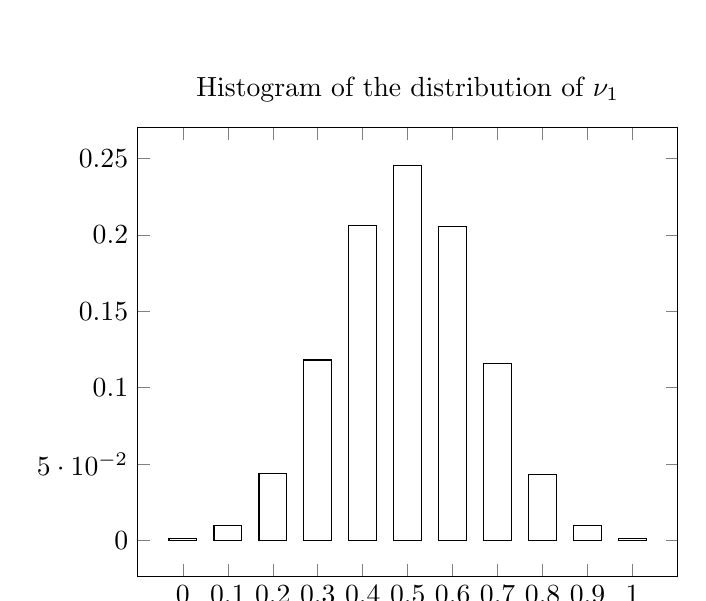
\begin{tikzpicture}[scale=1]
\begin{axis} [
	symbolic x coords={0,0.1,0.2,0.3,0.4,0.5,0.6,0.7,0.8,0.9,1},
		title = Histogram of the distribution of $\nu_1$,
		xtick = data
		]
\addplot[ybar] coordinates
	{(0,0.00101) (0.1,0.00965) (0.2,0.04372) (0.3,0.11813) (0.4,0.20601) (0.5,0.24572) (0.6,0.20578) (0.7,0.11614) (0.8,0.04288) (0.9,0.00992) (1,0.00104)  };
\end{axis}
\end{tikzpicture}
\par

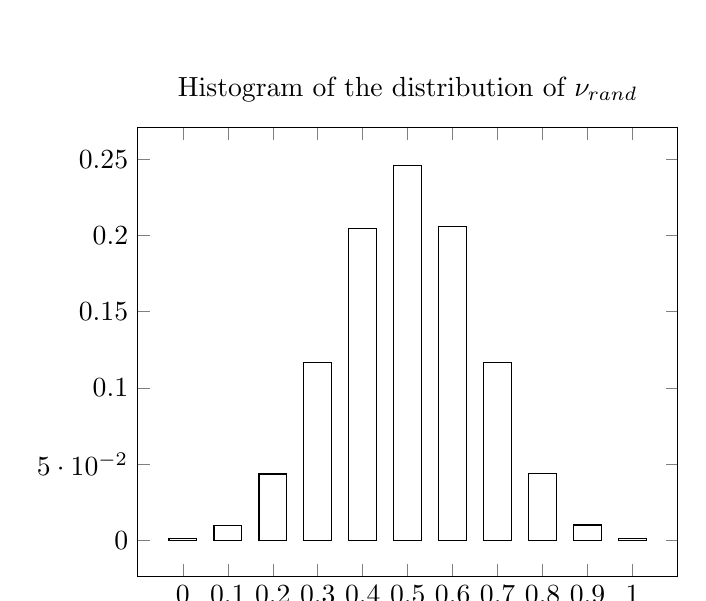
\begin{tikzpicture}[scale=1]
\begin{axis} [
	symbolic x coords={0,0.1,0.2,0.3,0.4,0.5,0.6,0.7,0.8,0.9,1},
		title = Histogram of the distribution of $\nu_{rand}$,
		xtick = data
		]
\addplot[ybar] coordinates
	{(0,0.00099) (0.1,0.00998) (0.2,0.04355) (0.3,0.11674) (0.4,0.20469) (0.5,0.24612) (0.6,0.20598) (0.7,0.11696) (0.8,0.04394) (0.9,0.01007) (1,0.00098) };
\end{axis}
\end{tikzpicture}
\par

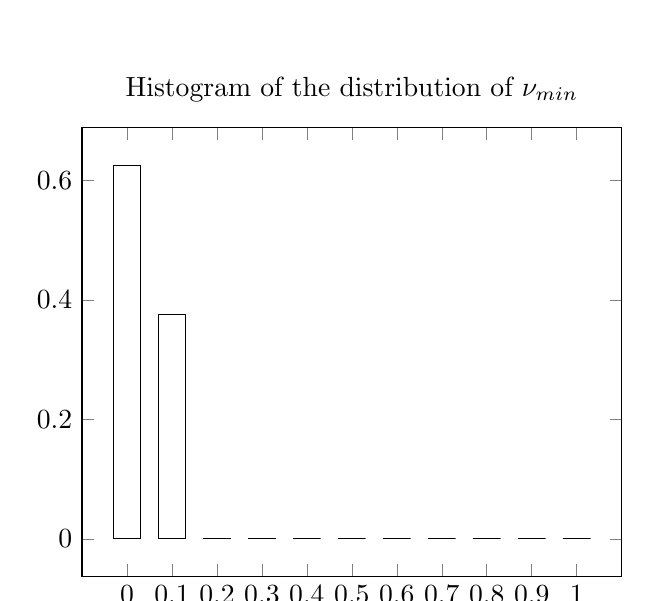
\begin{tikzpicture}[scale=1]
\begin{axis} [
	symbolic x coords={0,0.1,0.2,0.3,0.4,0.5,0.6,0.7,0.8,0.9,1},
		title = Histogram of the distribution of $\nu_{min}$,
		xtick = data
		]
\addplot[ybar] coordinates
	{(0,0.62518) (0.1,0.3748) (0.2, 0.00002) (0.3,0.0) (0.4,0.0) (0.5,0.0) (0.6,0.0) (0.7,0.0) (0.8,0.0) (0.9,0.0) (1,0.0) };
\end{axis}
\end{tikzpicture}
\par
\end{center}

\indent (c) The plots of the scaled estimators are as follows, we used $0.25*exp(-20*(x-0.5)^2)$ instead of $2*exp(-20*(x-0.5)^2)$ to visualize the pattern between the real distribution of the data and the estimators.
\begin{center}
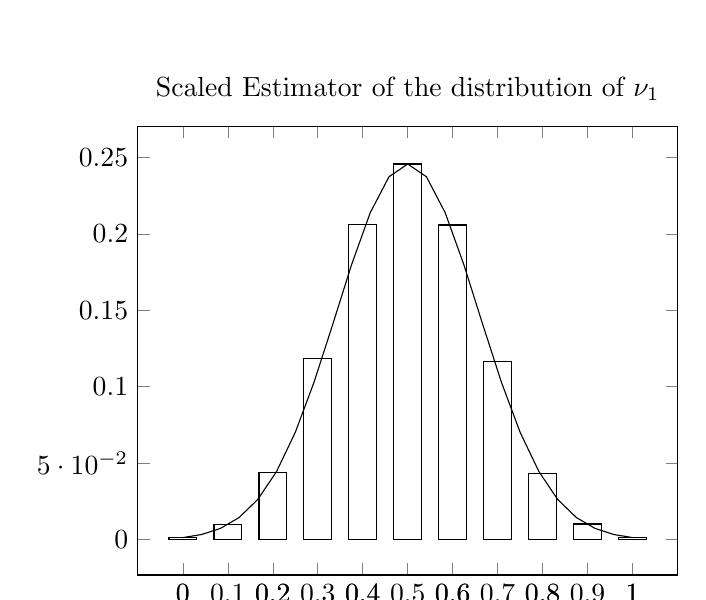
\begin{tikzpicture}[scale=1]
\begin{axis} [
	symbolic x coords={0,0.1,0.2,0.3,0.4,0.5,0.6,0.7,0.8,0.9,1},
		title = Scaled Estimator of the distribution of $\nu_1$,
		xtick = data ]
\addplot[ybar] coordinates
	{(0,0.00101) (0.1,0.00965) (0.2,0.04372) (0.3,0.11813) (0.4,0.20601) (0.5,0.24572) (0.6,0.20578) (0.7,0.11614) (0.8,0.04288) (0.9,0.00992) (1,0.00104)  };
\end{axis}
\begin{axis}[yticklabels={},tick style ={draw=none}]
\addplot[samples==200,domain=0:1]{0.25*exp{-20*(x-0.5)^2}};
\end{axis}
\end{tikzpicture}
\par

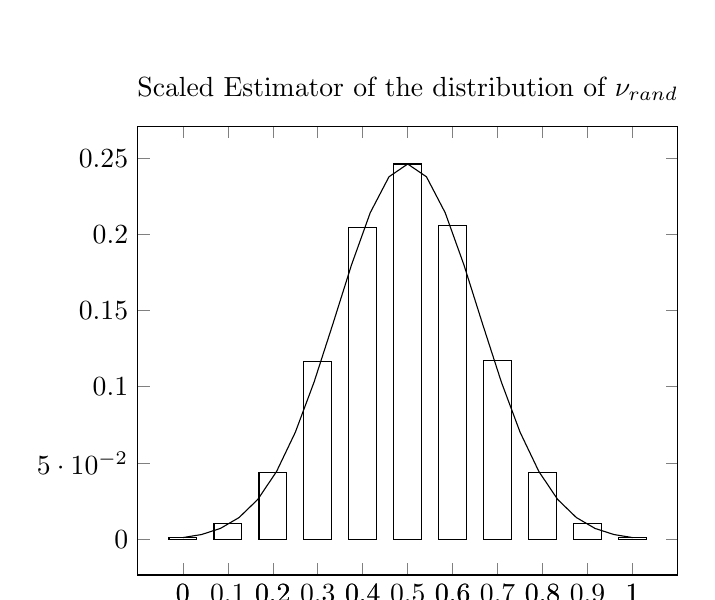
\begin{tikzpicture}[scale=1]
\begin{axis} [
	symbolic x coords={0,0.1,0.2,0.3,0.4,0.5,0.6,0.7,0.8,0.9,1},
		title = Scaled Estimator of the distribution of $\nu_{rand}$,
		xtick = data ]
\addplot[ybar] coordinates
	{(0,0.00099) (0.1,0.00998) (0.2,0.04355) (0.3,0.11674) (0.4,0.20469) (0.5,0.24612) (0.6,0.20598) (0.7,0.11696) (0.8,0.04394) (0.9,0.01007) (1,0.00098) };
\end{axis}
\begin{axis}[yticklabels={},tick style ={draw=none}]
\addplot[samples==200,domain=0:1]{0.25*exp{-20*(x-0.5)^2}};
\end{axis}
\end{tikzpicture}
\par

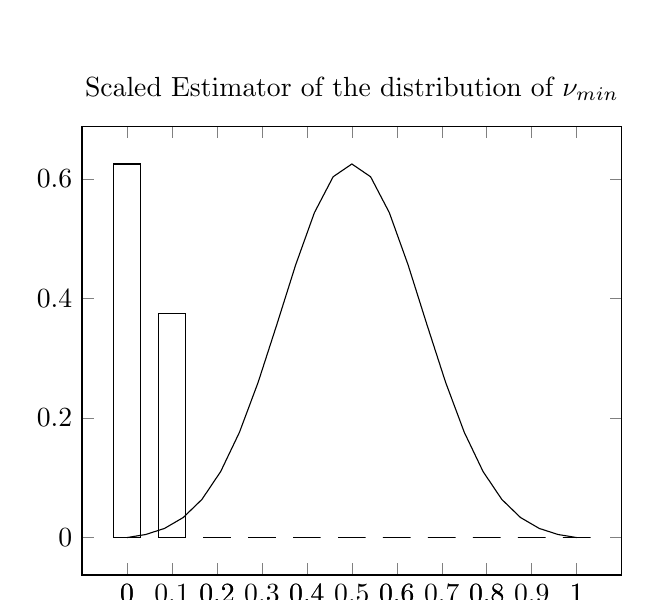
\begin{tikzpicture}[scale=1]
\begin{axis} [
	symbolic x coords={0,0.1,0.2,0.3,0.4,0.5,0.6,0.7,0.8,0.9,1},
		title = Scaled Estimator of the distribution of $\nu_{min}$,
		xtick = data ]
\addplot[ybar] coordinates
	{(0,0.62518) (0.1,0.3748) (0.2, 0.00002) (0.3,0.0) (0.4,0.0) (0.5,0.0) (0.6,0.0) (0.7,0.0) (0.8,0.0) (0.9,0.0) (1,0.0)  };
\end{axis}
\begin{axis}[yticklabels={},tick style ={draw=none}]
\addplot[samples==200,domain=0:1]{0.25*exp{-20*(x-0.5)^2}};
\end{axis}
\end{tikzpicture}
\par
\end{center}

\indent (d) Only coin $c_1$ and $c_{rand}$ obey the Hoeffding bound, while $c_{min}$ does not. $c_1$ follows the same pattern as $c_{rand}$ since they are randomly chosen coins. They are both fixed coins during the simulation process, thus obeys the Hoeffding bound. However, coin $c_{min}$ is not a fixed coin, it corresponds to the coin with minimum heads, since it's fixed before the data set was generated, the Hoeffding Inequality does not hold.\\
\indent (e) $c_1$ and $c_{rand}$ can represent multiple bins, in which each coin can be regarded as one bin, $h$ is fixed before a data set is generated. $c_{min}$ cannot represent bins, since it is not fixed, but it is closely related to the generated data set.\\

\noindent {\bf Exercise 1.11} \\\\
\indent (a) No. It cannot be guaranteed, there are 25 training examples, either case of  $p > 0.5 $, $p < 0.5$ or $p = 0.5$, the hypothesis produced by $S$ does not performs better than random on any point outside $\mathbb{D}$.\\
\indent (b) Yes, it is possible. If $p_{real} < 0.5$ and all training samples are labeled as $+1$, then the hypothesis produced by $C$ performs better than $S$.\\
\indent (c) Since $p = 0.9$, $h_1$ is better than $h_2$. So, if S produce a better hypothesis than C, S must pick $h_1$, which means there are at least $13$ examples that agree with $f(x) = +1$. Therefore, probability of S produce a better hypothesis than C is equals to the probability of there are no less than 13 $+1$ with in the $25$ examples given $p = 0.9$
\begin{align*}
	\mathbb{P} & =\sum_{i = 13}^{25} {25 \choose i}(0.9)^i(0.1)^{(25-i)} = 0.999999837
\end{align*}

\noindent {\bf Exercise 1.12} \\\\
\indent (c) should be the best. The feasibility of learning is to verify $E_{out}(g) \approx E_{in}(g)$ and $E_{in}(g) \approx 0$. 4000 data points is too small for the above condition to hold. Even if $E_{in}(g) \approx 0$, there's no guarantee that $E_{out}(g) \approx E_{in}(g)$ with high probability.\\

\noindent {\bf Problem 1.3} \\\\
\indent (a) Since $\textbf{w}^*$ is an optimal set of weights which separates the data , $\textbf{w}^{*^{T}}\textbf{x}_n$ and $y_n$ has the same sign for $n$ where $1\leq n \leq N $. Thus, $\displaystyle\rho = \min_{1\leq n\leq N}y_n(\textbf{w}^{*^{T}}\textbf{x}_n) > 0$ holds.\\
\indent (b) Since we know the update rule is 
\begin{center} $w(t) = w(t-1) + y(t-1)x(t-1)$\end{center} It follows that \begin{center} $w^T(t)w^*= w^T(t-1)w^* + w^*y(t-1)x(t-1)$\\$\geq w^T(t-1)w^* + min(y(t-1)(w^*x(t-1)))$\\$=w^T(t-1)w^* + \rho$\\$\geq w^T(t-2)w^* + \rho + \rho$ \\ $=w^T(t-2)w^* + 2\rho$\\ $\geq w^T(t-3)w^* + 3\rho $ \\ $\geq ...$ \\$\geq w^T(0)w^* + 6*\rho$\end{center} and we know $w(0) = 0$, thus \begin{center} $w^T(t)w^* \geq t\rho$\end{center}
\indent (c) Again, Since we know the update rule is 
\begin{center} $w(t) = w(t-1) + y(t-1)x(t-1)$\end{center} It follows that \begin{center} $||w(t)||^2 = ||w(t-1)||^2 + ||y(t-1)x(t-1)||^2 + 2y(t-1)w^T(t-1)x(t-1)$\end{center} We know $w(t-1)$ misclassifies $x(t-1)$, thus \begin{center} $y(t-1)w^T(t-1)x(t-1) < 0$\end{center}So, \begin{center} $||w(t)||^2 \leq ||w(t-1)||^2 + ||y(t-1)x(t-1)||^2 $ \\ $=||w(t-1)||^2 + ||x(t-1)||^2$ \end{center}
\indent (d) From part (c), we have  \begin{center} $||w(t)||^2 \leq ||w(t-1)||^2 + ||x(t-1)||^2$ \\ $\leq (||w(t-1)||^2 + ||x(t-1)||^2) + ||x(t-1)||^2$ \\ $\leq ... $ \\ $\leq ||w(0)||^2 + \sum_{n=1}^{t-1}||x(n)||^2$ \\ $=\sum_{n=1}^{t-1}||x(n)||^2$ \\ $\leq tR^2$\end{center} and $R = \max_{1\leq n\ leq N}||\textbf{x}_n||$\\\\
\indent (e) From part (d), since \begin{center} $||w(t)||^2 \leq tR^2||$ \\ $||w(t)|| \leq \sqrt{t}R$ \\ $\frac{w^T(t)}{||w(t)||}w^* \geq \frac{t\rho}{\sqrt{t}R} \geq\sqrt{t}\frac{\rho}{R}$\\ $\sqrt{t} \leq \frac{R}{\rho} \frac{w^T(t)}{||w(t)||}w^*$\end{center}And due to Cauchy Inequality $\alpha^T\beta \leq ||\alpha||||\beta||$: \begin{center}$\sqrt{t} \leq \frac{R}{\rho} \frac{||w(t)||||w^*||}{||w(t)||}$\\$\sqrt{t} \leq \frac{R||w^*||}{\rho}$\\$t \leq \frac{R^2||w^*||^2}{\rho^2}$\end{center}

\noindent {\bf Problem 1.7} \\\\
\indent (a)
\begin{center} For $\mu = 0.05$: \end{center}
\par N = 1 : $\displaystyle {10\choose0}0.05^0(1-0.05)^{10} = 0.5987$
\par N = 1,000 : $\displaystyle \mathbb{P} = 1-(1-{10\choose0}0.05^0(1-0.05)^{10})^{1000} = 1-2.6864\times10^{-397} \approx 1$
\par N = 1,000,000 : $\displaystyle \mathbb{P} = 1-(1-{10\choose0}0.05^0(1-0.05)^{10})^{1000000} = 1-1.519\times10^{-396571} \approx 1$
\begin{center} For $\mu = 0.8$: \end{center}
\par N = 1 : $\displaystyle {10\choose0}0.8^0(1-0.8)^{10} = 1.024\times10^{-7}$
\par N = 1,000 : $\displaystyle 1-(1-{10\choose0}0.8^0(1-0.8)^{10})^{1000} = 1.024\times10^{-4}$
\par N = 1,000,000 : $\displaystyle 1-(1-{10\choose0}0.8^0(1-0.8)^{10})^{1000000} = 0.097$\\\\
\indent (b) The distribution of $k$ is as follows:\\\\
\indent Since only 2 coins, either $|v_1 - \mu_1| > \epsilon$ or $|v_2 - \mu_2| > \epsilon$. \\\\
1) $\epsilon \in [0,1/6)$: coins are in $\{3\}$ thus $P = 1 - 0.3125^2 = 0.902$\\\\
2) $\epsilon \in [1/6,2/6)$: coins are in $\{2,3,4\}$ $P = 1 - (0.2344 + 0.3125 + 0.2344)^2 = 0.390$\\\\
3) $\epsilon \in [3/6,1)$: coins are in $\{1,2,3,4,5,6\}$ all cases have been excluded so $P = 0$
\begin{center}
\begin{tabular}{ |c|c|c|c|c|c|c|c| } 
 \hline
 k & 0 & 1 & 2 & 3 & 4 & 5 & 6 \\ 
 $|v-\mu |$ & 3/6 & 2/6 & 1/6 & 0 & 1/6 & 2/6 & 3/6 \\ 
 $\mathbb{P} |v - \mu|$ & 0.0156 & 0.0938 & 0.2344 & 0.3125 & 0.2344 & 0.0938 & 0.0156 \\ 
 \hline
\end{tabular}
\end{center}

\begin{center}
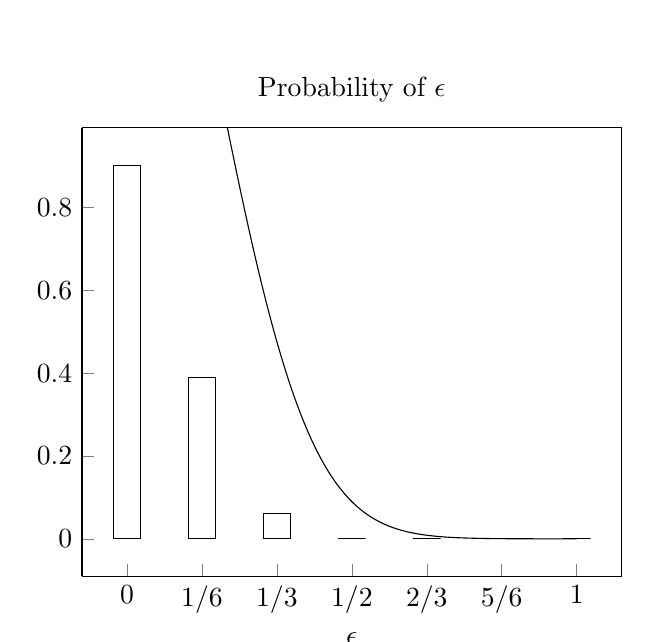
\begin{tikzpicture}[scale=1]
\begin{axis} [
	symbolic x coords={0, 1/6, 1/3, 1/2, 2/3, 5/6, 1},
	title = Probability of $\epsilon$,
		axis y line*=left,
		axis x line*=bottom,
		xtick = data,
		xlabel = $\epsilon$,
		]
\addplot[ybar] coordinates
	{(0, 0.90234375) (1/6, 0.3896484375) (1/3, 0.0615234375) (1/2, 0)(2/3, 0)(5/6, 0)(1, 0)};
\end{axis}
\begin{axis}[
	axis y line*=right,
	axis x line*=top,ymax = 1.1, xmax = 1.1, xmin = -0.1, ymin = -0.1,tick style ={draw=none},yticklabels={},xticklabels={}]
	\addplot[samples=200,domain=0:1]{2*exp(-12*(x)^2)};
\end{axis}
\end{tikzpicture}
\end{center}
\end{document}
